\begin{figure}[H]
	\centering
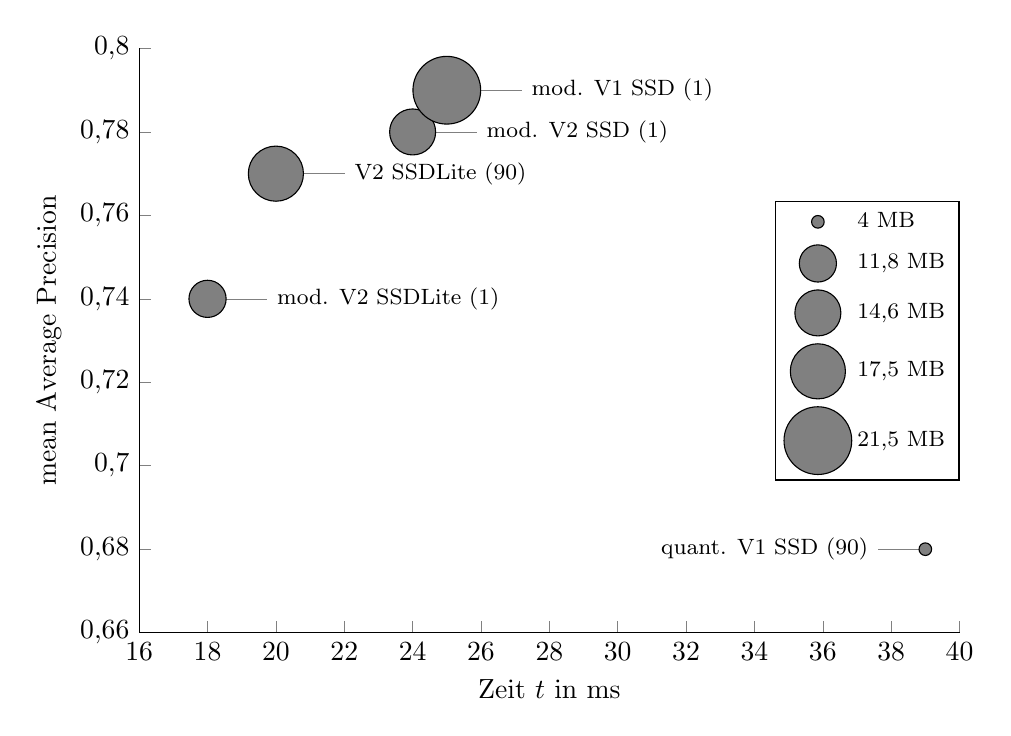
\begin{tikzpicture}
	\begin{axis}[
width=12cm,
height=9cm,
axis y line*=left,
ticklabel style={% gilt für x und y
	/pgf/number format/.cd,
	use comma,% Komma als Dezimaltrenner
	1000 sep = {}% keine Tausendertrennung 
},
xlabel={Zeit $t$ in ms},
ylabel={mean Average Precision},
axis x line*=bottom,
xmin=16, xmax=40, 
ymin=0.66, ymax=0.8,
%every axis plot/.append style={line width=1.0pt}
%legend pos=north east,
legend cell align={left},
legend style={row sep = 0.1cm,at={(1,0.5)},anchor=east} ,
]
\addlegendentry{\footnotesize 4 MB};
\addlegendentry{\footnotesize 11,8 MB};
\addlegendentry{\footnotesize 14,6 MB};
\addlegendentry{\footnotesize 17,5 MB};
\addlegendentry{\footnotesize 21,5 MB};
\addplot[only marks, mark options = {draw =black, scale = 0.04cm, fill = gray}] coordinates{(39,0.68)} node[xshift=0.1cm,pos=0,pin={[pin distance=0.58cm]left:{\footnotesize quant. V1 SSD (90)}}]{} ;
\addplot[only marks, mark options = {draw =black, scale = 0.118cm, fill = gray}] coordinates{(18,0.74)} node[xshift=-0.1cm,pos=0, pin={[pin distance=0.736cm]right:{\footnotesize mod. V2 SSDLite (1)}}]{} ;
\addplot[only marks, mark options = {draw =black, scale = 0.146cm, fill = gray}] coordinates{(24,0.78)} node[xshift=-0.1cm,pos=0, pin={[pin distance=0.792cm]right:{\footnotesize mod. V2 SSD (1)}}]{} ;
\addplot[only marks, mark options = {draw =black, scale = 0.175cm, fill = gray}] coordinates{(20,0.77)} node[xshift=-0.1cm,pos=0, pin={[pin distance=0.85cm]right:{\footnotesize  V2 SSDLite (90)}}]{} ;

\addplot[only marks, mark options = {draw =black, scale = 0.215cm, fill = gray}] coordinates{(25,0.79)} node[xshift=-0.1cm,pos=0, pin={[pin distance=0.93cm]right:{\footnotesize mod. V1 SSD (1)}}]{} ;
\end{axis}
\end{tikzpicture}
	\caption{Vergleich aller untersuchten \textit{MobileNet} Architekturen. Das Diagramm stellt die \textit{mean Average Precision} aufgetragen über die gemessene Rechenzeit dar. Gezeigt ist der Test auf dem integrierten Rechner des ALFs in Anwendung auf den eigenen Datensatz.   }
\label{fig: komplettvergleich}


\end{figure}